\documentclass{standalone}
\usepackage[T1]{fontenc}
\usepackage[latin2]{inputenc}
\usepackage[english]{babel}
\usepackage{tikz}
\usepackage{times}
\usetikzlibrary{calc,through,backgrounds,positioning,fit}
\usetikzlibrary{shapes,arrows,shadows}
 
\begin{document}
 
\tikzstyle{place}=[shape=circle, draw, minimum height=10mm]
\tikzstyle{trig}=[shape=circle, draw, dashed, minimum height=10mm]
\tikzstyle{trans}=[shape=rectangle, draw, minimum height=6mm, minimum width=12mm]
 
\centering
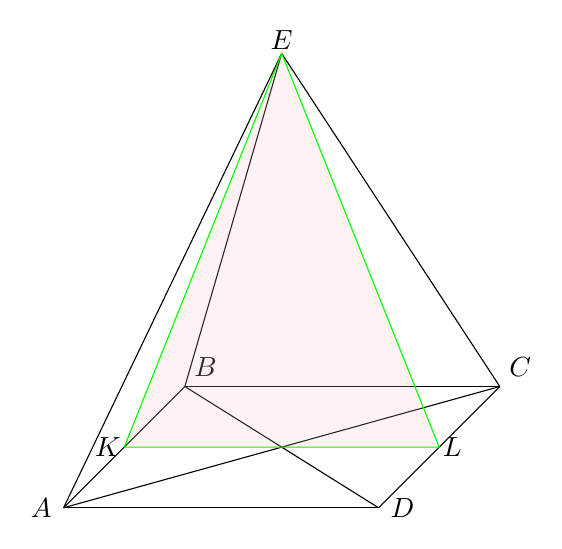
\begin{tikzpicture}[scale=1,inner sep=0.4mm]
\coordinate (A) at (0,0,4);
\coordinate (B) at (0,0,0);
\coordinate (C) at (4,0,0);
\coordinate (D) at (4,0,4);
\coordinate (E) at (2,5,2);
\coordinate (K) at (0,0,2);
\coordinate (L) at (4,0,2);

\draw(A)node [left=3pt] {$A$}-- (B) node[above right=3pt] {$B$} ;
\draw(A) -- (C) node[above right=3pt] {$C$};
\draw(A) -- (D)node [right=3pt] {$D$};
\draw(B) -- (C);
\draw(B) -- (D);
\draw(D) -- (C);
\draw(A) -- (E);
\draw(B) -- (E);
\draw(C) -- (E);
\draw(E) -- (E);


\draw [green, fill=pink, fill opacity=0.2] (K)--(L)--(E)--(K); 
\node at (K) [left] {$K$};
\node at (L) [right] {$L$};
\node at (E) [above] {$E$};

\end{tikzpicture}
 
\end{document}